\section{Technologie}\label{architektur.technologie}
%TODO: Lead
	\subsection{Server}
%TODO: Lead

		\subsubsection{Evaluation}\label{serverEvaluation}
			Die Servertechnologie stellt eine entscheidende Komponente dar, 
			ihre Wahl ist von entsprechender Tragweite für andere Komponenten des Projektes.
			Aus diesem Grund haben wir sie ausführlich evaluiert.
			
			\begin{enumerate}
				\item Schritt: Gemeinsame Definition von Kriterien und möglichen Servertechnologien.
				\item Schritt: Separate Festlegung der Gewichtung der Kriterien sowie Definition der Matrix Kriterium/Servertechnologie mit der persönliche Schätzung, wie stark jede Servertechnologie das entsprechende Kriterium erfüllt.
				\item Schritt: Zusammenführung der persönlichen Ergebnisse zu Gesamtergebnis
			\end{enumerate}
		
			\begin{figure}[H]
				\begin{minipage}[b]{\linewidth}
					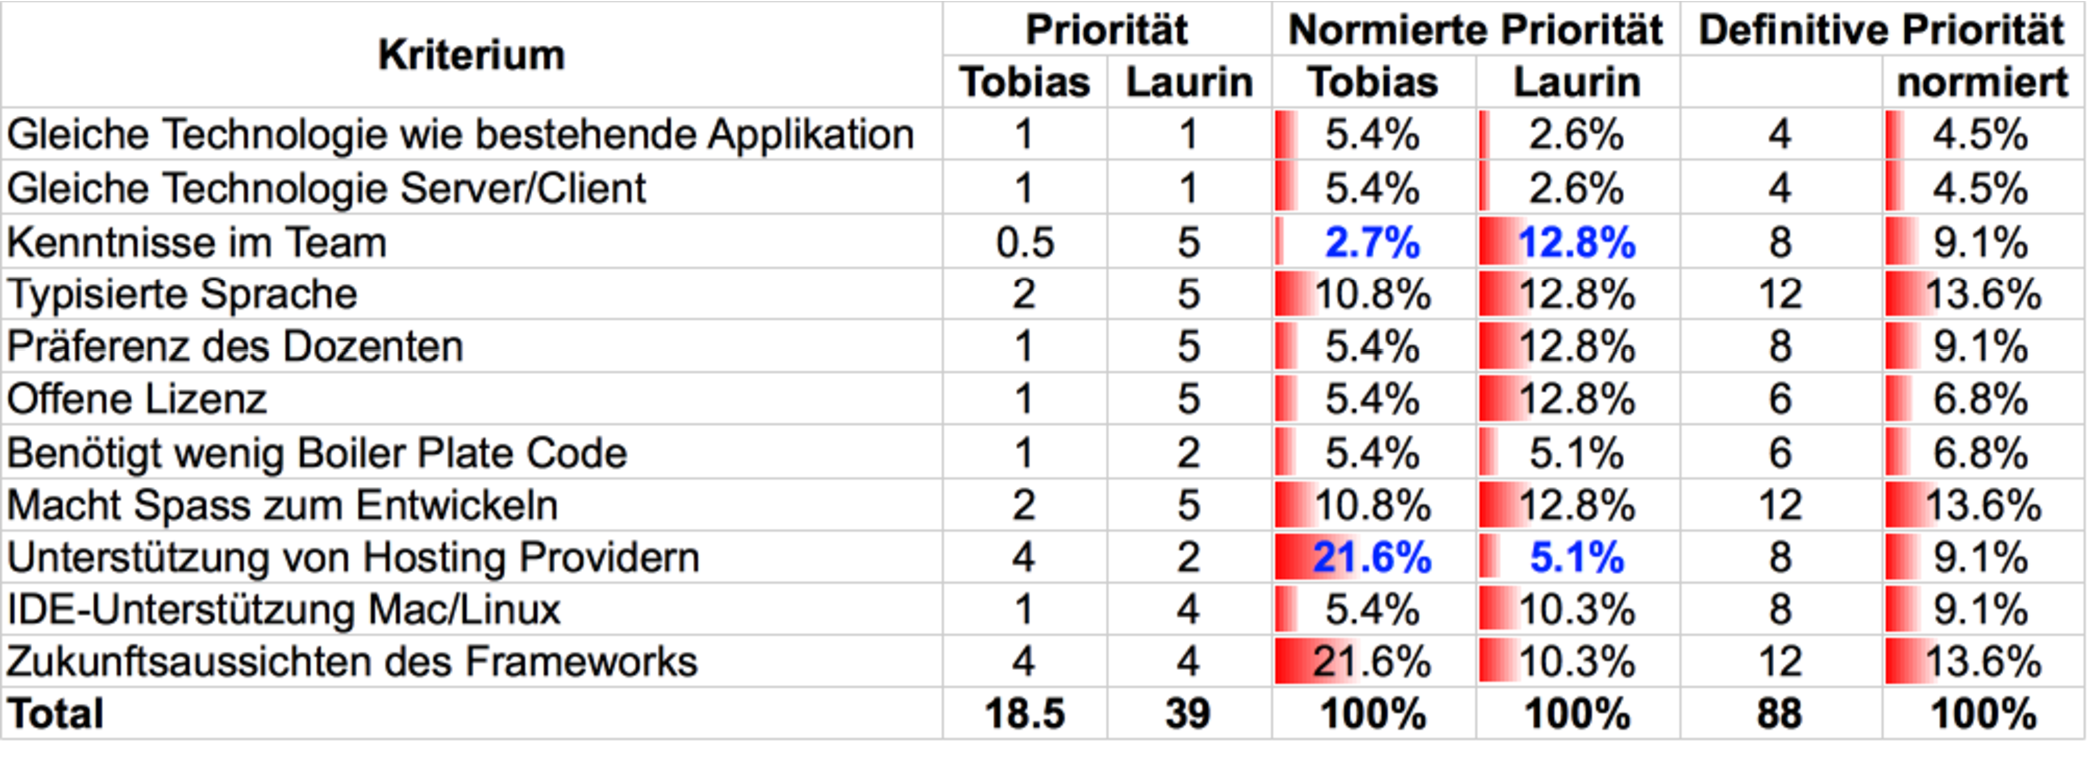
\includegraphics[width=\textwidth]{media/spreadsheets/ServertechnologieVergleichPrioritaetsfinding.pdf}
					\centering
					\caption{Servertechnologie-Vergleich: Prioritätsfindung}
					\label{fig:ServertechnologieVergleichPrioritaetsfinding}
				\end{minipage}
			\end{figure}
			
			Abbildung~\ref{fig:ServertechnologieVergleichPrioritaetsfinding} zeigt den Prozess der Prioritätsfindung.
			Wie bereits erwähnt, haben wir zuerst die Kriterien definiert und 
			anschliessend je separat Prioritäten für jedes Kriterium festgelegt.
			Da wir verschiedene Skalen verwendet haben, haben wir unsere Punkte noch zu 100\% normiert.
			Und aus diesen zwei Werten haben wir in gemeinsamer Diskussion die definitive Priorität erstellt.
			Dies hat meist problemlos funktioniert, ausser bei den Punkten "<Kenntnisse im Team"> und "<Unterstützung von Hosting Providern"> (blau markiert) hatten wir zu Beginn nennenswerte Unterschiede.
			Bei diesen Punkten haben wir dann in der gemeinsamen Diskussion einen Wert festgelegt.
		
			\begin{figure}[H]
				\begin{minipage}[b]{\linewidth}
					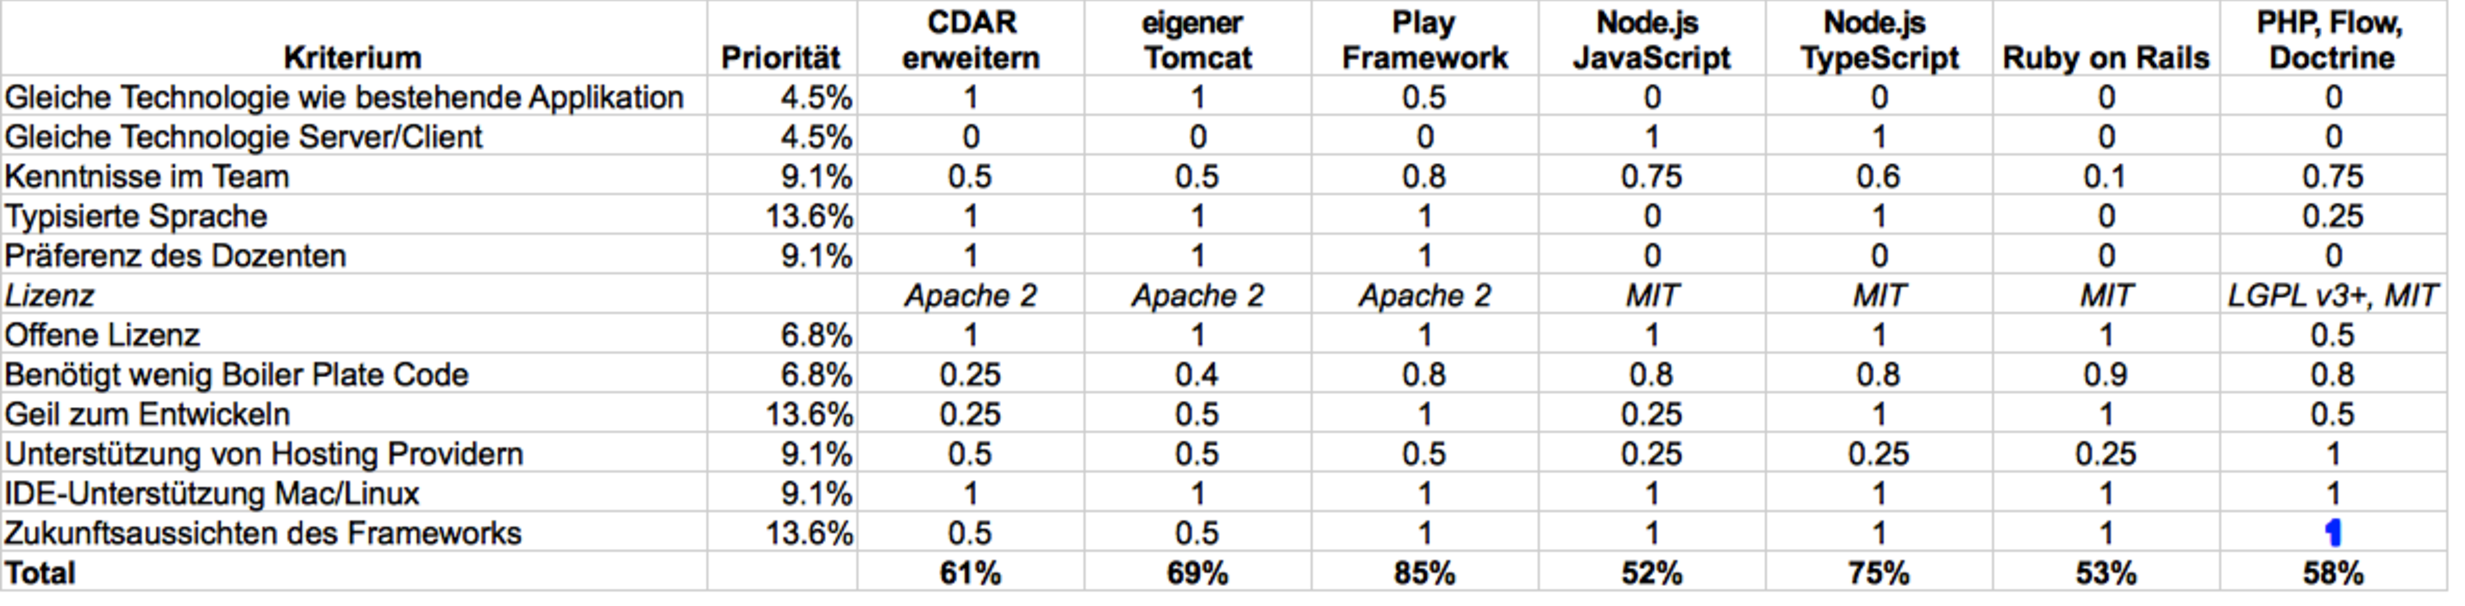
\includegraphics[width=\textwidth]{media/spreadsheets/ServertechnologieVergleichVergleichDerTechnologien.pdf}
					\centering
					\caption{Servertechnologie-Vergleich: Vergleich der Technologien}
					\label{fig:ServertechnologieVergleichVergleichDerTechnologien.pdf}
				\end{minipage}
			\end{figure}
			
			Abbildung~\ref{fig:ServertechnologieVergleichVergleichDerTechnologien.pdf} zeigt den Vergleich der einzeln evaluierten Servertechnologien.
			Auch hier haben wir zuerst je separat die Schätzung gemacht und dann verglichen.
			Bei diesem Vergleich haben wir gar noch ähnlichere Werte gewählt, lediglich bei den Zukunftsaussichten von PHP, Flow und Doctrine (blau markiert) hatten wir nennenswert unterschiedliche Ansichten.
			
			\begin{figure}
					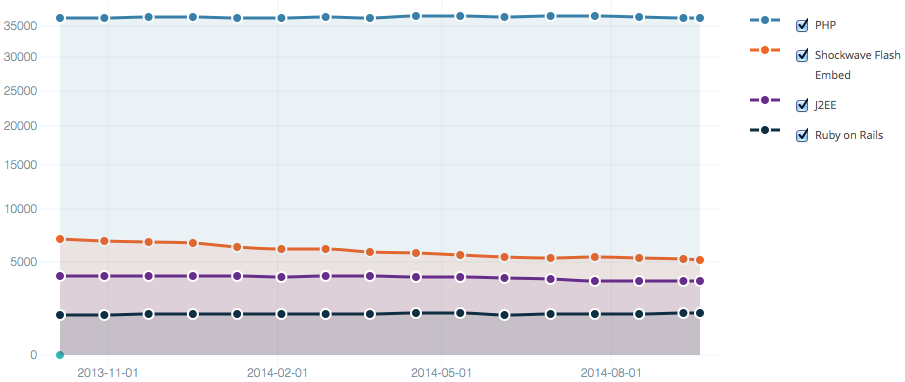
\includegraphics[width=\textwidth]{media/img/EntwicklungVonWebserverTechnologien.png}
					\centering
					\caption{Entwicklung von Webserver"=Technologien der Top 10'000 Sites \cite{builtwith_pty_ltd_framework_2014}}
					\label{fig:EntwicklungVonWebserverTechnologien}
			\end{figure}
			
			Schlussendlich haben wir uns da nach Recherchen auf eine "<1"> geeinigt, weil entgegen den Erwartungen von Laurin Murer sich die Verbreitung von PHP (auch bei grösseren Seiten) kaum verändert hat.
			Als Beispiel für eine Technologie, die immer weniger eingesetzt wird und in den nächsten Jahren verschwinden wird, haben wir Shockwave Flash herangezogen, welche, wie in Abbildung~\ref{fig:EntwicklungVonWebserverTechnologien} sichtbar, im letzten Jahr deutlich an Boden verloren hat.
			Im Vergleich dazu ist PHP sehr gut im Markt vertreten und hat auch eine äusserst konstante Verbreitung.
			Deshalb und unter dem Gesichtspunkt der soliden Konzepte, 
			die den in den letzten Jahren entstandenen modernen PHP Frameworks wie Doctrine und Flow zugrunde liegen, sehen wir da auch das Fortbestehen für diese Technologien gegeben.
			
			\begin{figure}[H]
				\begin{minipage}[b]{\linewidth}
					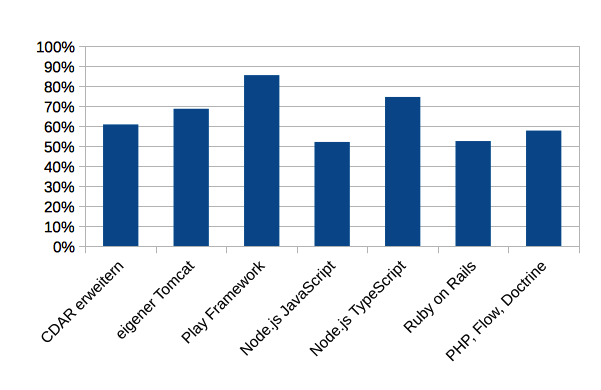
\includegraphics[width=\textwidth]{media/spreadsheets/ServertechnologieVergleichVergleichDerTechnologienDiagramm.png}
					\centering
					\caption{Ergebnis Servertechnologie-Vergleich}
					\label{fig:ErgebnisServertechnologieVergleich}
				\end{minipage}
			\end{figure}
			
			Schlussendlich haben wir für jede Technologie das Total der Punkte berechnet (Punkte jedes Kriteriums multipliziert mit seiner Priorität). in Abbildung~\ref{fig:ErgebnisServertechnologieVergleich} zeigt man das finale Ergebnis. Aufgrund diesem haben wir uns für das Play Framework entschieden. Eine Alternative wäre noch Node.js mit TypeScript gewesen, doch dies hat bereits 10\%-Punkte weniger erreicht.
			
			
		\decision{
			\decisionHeader{TEC-SERVER}{Servertechnologie}{Technologie}{Server}
		}{
			\decisionContent{Play Framework}
			{Welche Servertechnologie soll eingesetzt werden?}
			{keine Speziellen}
			{Von der Servertechnologie hängen unter Anderem die Entscheidungen für Server und Persistenz Framework ab.}
			{\cdar\ erweitern, eigener Tomcat, Node.js+JS, Node.js+TS, Ruby, PHP}
			{			
				\begin{itemize}
					\item Das Play Framework basiert auch auf Java, wie das bestehende \cdar.
					\item Ein Teammitglied hat bereits Erfahrungen mit dem Framework gemacht.
					\item Das andere Teammitglied kennt die zugrundeliegende Sprache (Java).
					\item Der Betreuer hat eine Präferenz für Java.
					\item Das Play Framework benötigt wenig Boilerplate-Code.
					\item Es sprechen keine zwingenden Gründe dagegen (wie beispielsweise zu stark einschränkende Lizenzen).
					\item Das Play Framework ist angenehm zum Entwickeln für die Entwickler: gegebener Spass-Faktor, Vermeidung von Fehlern, Unterstützung im Erreichen von guter Code Qualität.
					\item Im IFS der HSR ist Know How zum Play Framework vorhanden (M. Stocker).
				\end{itemize}
			}
			{keine Speziellen}
			{keine}
			{keine}
		}

		\subsubsection{Play Framework}
			Kapitel~\ref{serverEvaluation} erläutert den Hintergrund der Entscheidung für das Play Framework. 
			
			Wikipedia beschreibt das Play Framework wie folgt:
			\begin{quote}
				"<Play is an open source web application framework, written in Scala and Java, which follows the model–view–controller (MVC) architectural pattern. It aims to optimize developer productivity by using convention over configuration, hot code reloading and display of errors in the browser."> \cite{builtwith_pty_ltd_framework_2014}
			\end{quote}

			

	\subsection{Client}
%TODO: Lead
		\subsubsection{Sprache}
%TODO: Lead
		\decision{
			\decisionHeader{TEC-CLIENT-LANG}{Clientseitige Programmiersprache}{Technologie}{Sprache}
		}{
			\decisionContent{TypeScript}
			{Welche Sprache soll clientseitig verwendet werden?}
			{keine Speziellen}
			{Diese Entscheidung beeinflusst die Optionen der Client Frameworks und sie entscheidet, ob die gewählte Sprache gutes Code-Schreiben unterstützt, wenig fehleranfällig ist und Fehler frühzeitig erkannt werden können, oder ob die Sprache Fehler begünstigt und damit die Qualität des Codes verringert.}
			{
				\begin{description}
					\item[JavaScript] \
						\begin{description}
							\item[Vorteile] UI der bestehenden Applikation ist auch in JavaScript geschrieben
							\item[Nachteile] Fehler tauchen erst zur Runtime auf, sprachspezifische Besonderheiten, die Fehler begünstigen
						\end{description}
					\item[Dart] \
						\begin{description}
							\item[Vorteile] Moderne, optional typisierte, kompilierte Programmiersprache (wird zu JS kompiliert)
							\item[Nachteile] Benötigt Dart VM oder Dart-to-JS Transcompiler, wenig verbreitet
						\end{description}
				\end{description}
			}{TypeScript wird zu JavaScript kompiliert, sodass die Vorteile beide Sprachen kombiniert werden. TypeScript versucht, möglichst den Standard zukünftiger ECMA-Script Versionen einzuhalten, sodass die Kompatibilität immer gewährleistet und die Syntax möglichst ähnlich bleiben soll.
			\begin{description}
				\item[Vorteile] Optisch besser lesbar als JavaScript, verhindert bekannte, häufige Probleme in JavaScript wie z.B. das ungewohnte verhalten von "<this">, verbessert die Codequalität gegenüber JavaScript massiv, da viele Fehler zur Kompilierzeit gefunden werden
				\item[Nachteile] Erfordert TSC-Compiler, Code Overhead bei Inheritance
			\end{description}
			}{keine Speziellen}
			{Die Entwicklungsumgebung benötigt Node.js für den TypeScript Compiler.}
			{keine}
		}
			
			
		\subsubsection{Architektur-Framework}
			\decision{
				\decisionHeader{TEC-CLIENT-FW}{Clientseitiges Applikationsframework}{Technologie}{Framework}
			}{
				\decisionContent{AngularJS}
				{Welches Applikationsframework soll clientseitig eingesetzt werden?}
				{keine Speziellen}
				{Diese Entscheidung legt den Grundstein für den technologischen Aufbau der clientseitigen Applikation und soll ein Framework evaluieren, das Templating und Two-Way-Binding mit UI Komponenten unterstützen, um dies nicht selbst implementieren zu müssen.}
				{
					\begin{description}
						\item[EmberJS] \
							\begin{description}
								\item[Vorteile] Sehr modular und anpassbar, weniger Overhead als AngularJS
								\item[Nachteile] Bringt wesentlich weniger mit als Angular JS, mehr Eigenaufwand notwendig, kann nur einfache Datentypen an UI Elemente binden
							\end{description}
						\item[Kein Framework] \
							\begin{description}
								\item[Vorteile] Vollständig freie Architekturgestaltung
								\item[Nachteile] Hoher Implementationsaufwand ohne Gewinn
							\end{description}
					\end{description}
				}
				{Angular JS ist ein bekanntes MVW\footnote{Model View Whatever:
				Fasst MVC, MVP und andere ähnliche Strukturierungspatterns zusammen, wird manchmal auch "<MV*\hspace{0.05em}"> genannt.
				}- und Templating Framework, erlaubt eine saubere Trennung von Logik
				und Darstellung und bindet ViewModel-Eigenschaften und "=Funktionen ans Template.
				Dadurch lassen sich Observerkonstrukte sparen.
				AngularJS ist stabil, zuverlässig, gut erweiterbar und bringt von sich aus schon sehr viel mit gegenüber EmberJS. Es wurde auch schon für die bestehende Applikation (\cdar) eingesetzt.}
				{keine Speziellen}
				{Die Serverkomponente muss eine Schnittstelle bieten, über die die Clientapplikation Daten austauschen kann.}
				{keine}
			}
		
			
			\subsubsection{JavScript Autoloading}
				Ursprünglich war die Idee, Require.js als Autoloader zu benutzen.
				Require.js bietet nebst Vorteilen wie Namespacing und Autoloading leider den grossen Nachteil,
				dass jedes Skript einzeln asynchron vom Client angefordert wird, 
				was insbesondere bei grösseren Round-Trip-Times die Applikation spürbar verlangsamt.
				Aus diesem Grund wurde entschieden, 
				auf die Bordmittel von TypeScript zur Strukturierung zu setzen (Modules/Packages) 
				und die verschiedenen Skripte bereits beim Kompilieren zusammenzuführen.
				

		\subsection{UI Frameworks}
			\subsubsection{Less}
				Less\footnote{CSS Pre-Prozessor: \url{http://lesscss.org/}} wird als CSS Generator eingesetzt, da es den CSS Code stark verschlankt und Vorteile wie Variablen und Mixins bietet.
				Less wird serverseitig kompiliert um den Client zu entlasten.
				
		\subsection{Testing}
			Testing Framework Anforderungen:
			\begin{itemize}
				\item Einfach einzubinden
				\item Einfach zu erweitern
				\item Bekannte Benutzung mit Tests und Asserts
				\item Möglichkeit zur Anbindung eines Build Tools
			\end{itemize}

			\subsubsection{JsUnit / QUnit} %TODO: noch aktuell?
				JsUnit wie QUnit arbeiten mit einem realen Browser (keine Browsersimulation), 
				sind einfach zu handhaben und bieten typische Assert-Syntax.
				
				
